\documentclass[12pt, titlepage]{article}
\usepackage{graphicx}
\usepackage{booktabs}
\usepackage{tabularx}
\usepackage{hyperref}
\hypersetup{
    colorlinks,
    citecolor=black,
    filecolor=black,
    linkcolor=red,
    urlcolor=blue
}
\usepackage[round]{natbib}

\usepackage{color}

\newif\ifcomments\commentstrue

\ifcomments
\newcommand{\authornote}[3]{\textcolor{#1}{[#3 ---#2]}}
\newcommand{\todo}[1]{\textcolor{red}{[TODO: #1]}}
\else
\newcommand{\authornote}[3]{}
\newcommand{\todo}[1]{}
\fi

\newcommand{\wss}[1]{\authornote{blue}{SS}{#1}} 
\newcommand{\plt}[1]{\authornote{magenta}{TPLT}{#1}} %For explanation of the template
\newcommand{\an}[1]{\authornote{cyan}{Author}{#1}}

%% Common Parts

\newcommand{\progname}{ProgName} % PUT YOUR PROGRAM NAME HERE %Every program
                                % should have a name


\begin{document}

\title{Unit Verification and Validation Plan for Stoichiometry Mass-Mass Program } 
\author{Deemah Alomair}
\date{\today}
	
\maketitle

\pagenumbering{roman}

\section{Revision History}

\begin{tabularx}{\textwidth}{p{3cm}p{2cm}X}
\toprule {\bf Date} & {\bf Version} & {\bf Notes}\\
\midrule
26/12/2019 & 1.0 & First version of document\\
\bottomrule
\end{tabularx}

~\newpage

\tableofcontents

\listoftables 

\listoffigures
\newpage

\section{Symbols, Abbreviations and Acronyms}

\renewcommand{\arraystretch}{1.2}
\begin{tabular}{l l} 
  \toprule		
  \textbf{symbol} & \textbf{description}\\
  \midrule 
  SRS & Software Requirements Specification \\
  SMMP & Stoichiometry Mass-Mass Program \\
  T & Test \\
  \bottomrule
\end{tabular}\\


\newpage

\pagenumbering{arabic}

\section{General Information}

This section gives an overview of purpose of this document. In addition, describe the scope of the unit testing that will be carried on throughout the testing phase. 

\subsection{Purpose}

The main purpose of this document is to build verification and validation plan for Stoichiometry Mass-Mass Program, provide  description about the unit testing that will be carried out on SMMP, and check whether each SMMP function meets the SRS and fulfill its intended purpose. This document will be used as the reference and guidance for testing SMMP.


\subsection{Scope}
\begin{itemize}
\item The tests outlined in this document are limited to the verification of the requirements given in the SMMP SRS. 
\item The tests outlined in this document will include dynamic tests.
\item The tests outlined in this document will include manual and automated tests.
\item The tests outlined in this document will include integration testing.
\item The tests outlined in this document will include parallel testing in limited basis.
\item The SMMP software will be written in Python. The testing of implementations in other languages will not be considered in this document.

\end{itemize}

\section{Plan}
	
\subsection{Verification and Validation Team}

The test team includes the following members:
\begin{itemize}
\item Main contributor: Deemah Alomair.
\item Primary reviewers: Dr. Spencer Smith, Sharon Wu.
\item Secondary reviewers: Bo Cao, Ao Dong, Peter Michalski.
\end{itemize}

\subsection{Automated Testing and Verification Tools}

The automated testing for SMMP will be carried out using coverage testing. PyCharm environment provides coverage testing package which will be used.



\subsection{Non-Testing Based Verification}

Not Applicable. 


\section{Unit Test Description}

This unit test description has been built to summarize all the unit tests that will be conducted in testing phase for each module individual functions. all modules related functions can be found in MIS document .

\subsection{Tests for Functional Requirements}

\subsubsection{input conversion test}

 First module will cover all individual functions in the first part of the SMMP which is converting user input into chemical reaction parameter.. 

\begin{enumerate}

\item{\bf T1: get number of chemical reaction elements \\}

Type: Functional, dynamic, Manual.
					
Initial State: Not Applicable. 
					
Input: user must input at least two chemical reactants and one product 
\begin{table}[h!]
\centering
\resizebox{\textwidth}{!}{\begin{tabular}{|c|c|c|}
\hline
input & example & output  \\
\hline
one reactant and products & $H_2$O $\rightarrow$ $H_2$ + $O_2$ & error massage \\ \hline
two reactant and no product & $H_2$ + $O_2$ $\rightarrow$ & error massage \\ \hline
two reactant and one product  & $H_2$ + $O_2$ $\rightarrow$ $H_2$O & accepted\\ \hline
two reactant and two product  & Fe$Cl_3$ + MgO $\rightarrow$ $Fe_2$$O_3$ + Mg$Cl_2$ & accepted \\ \hline
\hline
\end{tabular}}
\caption{Input number of elements possible entries and its corresponding outputs }
\label{elementsnumber}
\end{table}

Test Case Derivation: the expected entry is chemical reaction with at least two reactants and one product. 

How test will be performed: 
\begin{itemize}
\item the user will choose an elements from drop down menus using GUI widget for each reactant and product
\item the system will check if user choose at least one element for reactant 1, reactant 2 and product 1 to processed. 
\item if user did not fulfill the minimum requirement system will show up an error massage indicating that. 
\end{itemize}

\item{\bf T2: get name of chemical reaction elements \\}

Type: Functional, dynamic, Manual.
					
Initial State: Not Applicable. 
					
Input: user must input an element in both side of chemical reaction.

\begin{table}[h!]
\centering
\resizebox{\textwidth}{!}{\begin{tabular}{|c|c|c|}
\hline
input & output & explenation   \\
\hline
$H_2$ + $O_2$ $\rightarrow$ $H_2O$ & accepted  & H , O in both side of the reaction  \\ \hline
Fe$Cl_3$ + MgO $\rightarrow$ $Fe_2$$O_3$ & error massage & Mg is in reactant side but not in product side \\ \hline
$CO_2$ + O  $\rightarrow$ C$H_4$ + $O_2$ & error massage & H is in product side but not reactant side  \\ \hline
\hline
\end{tabular}}
\caption{Input name of element possible entries and its corresponding outputs }
\label{elementname}
\end{table}

Test Case Derivation: the expected entry is consistent chemical reaction where each element entered the reaction must produced from the reaction. 

How test will be performed: 
\begin{itemize}
\item the user will enter an elements from drop down menus using GUI widget for each reactant and product
\item the system will check if user enter the element in both sides of the reaction to processed. 
\item if user did not fulfill the minimum requirement system will show up an error massage indicating that. 
\end{itemize}

\item{\bf T3: get atom value of chemical reaction elements \\}

Control: Functional, dynamic, Manual.
					
Initial State: atom value = 0 if no element has been selected.
					
Input: 
atom value: 
\begin{table}[h!]
\centering
\begin{tabular}{|c|c|}
\hline
atom value & response  \\
\hline
atom value $\notin$ number  & error massage \\ \hline
atom value $\leq$ 0& error massage \\ \hline
atom value $>$ 0  & accepted\\ \hline
\hline
\end{tabular}
\caption{Input atom possible value's level}
\label{atom}
\end{table}
	
Output: error massage indicating that atom value is not a number or atom value $\leq$ 0. 

Test Case Derivation: the expected value is chemical element selected from a menu and atom value belongs to positive integer number. 

How test will be performed: 
\begin{itemize}
\item the system will get the values. 
\item the system will ensure user has already selected an element. 
\item process the atom value to ensure it's a number. if not error massage will be shown.
\item if its a number it will test if its greater than 0 or not.  if not error massage will be shown.
\end{itemize}

\item{\bf T4: get Mass Input \\}

Control: Functional, dynamic, Manual.
					
Initial State: Not Applicable.
					
Input: 
\begin{table}[h!]
\centering
\begin{tabular}{|c|c|}
\hline
input & response  \\
\hline
Mass $\notin$ number  & error massage \\ \hline
Mass $\leq$ 0& error massage \\ \hline
Mass $>$ 0  & accepted\\ \hline
\hline
\end{tabular}
\caption{Input mass possible value's level }
\label{mass}
\end{table}

Output: error massage indicating that mass value is not a number or mass value $\leq$ 0. 

Test Case Derivation: the expected value is a positive integer number. 
					
How test will be performed: 
\begin{itemize}
\item the system will get the value. 
\item process the value to ensure it's a number. if not error massage will be shown.
\item if its a number it will test if its greater than 0 or not.  if not error massage will be shown.
\end{itemize}

\item{\bf T5: get reactant of known Mass  \\}

Control: Functional, dynamic, Manual.
					
Initial State: Not Applicable.
					
Input: reactant number of known mass from drop down menu (1 or 2) 

Output: error massage indicating that reactant number is not chosen.

Test Case Derivation: the expected value is to choose which reactant the known mass belong to. . 
					
How test will be performed: 
the system will check if user choose the number of known reactant mass from drop down menu through GUI widget. if not error massage will be shown indicating that he need to choose from the menu before calculating the mass. 

\end{enumerate}

\subsubsection{Calculation Method Tests}

\paragraph{Balancing Calculation Tests}

\begin{enumerate}

\item{\bf T6: Count total number of atoms for each element in each side\\}

Control: Functional, dynamic, Manual.
					
Initial State: N.A
					
Input: Fe$Cl_3$ + MgO $\rightarrow$ $Fe_2$$O_3$ + Mg$Cl_2$ 

output: Reactants= [Fe:1, Cl:3 , Mg:1, O:1] , products = [Fe:2, Cl:2 , Mg:1, O:3] 
 
Test Case Derivation: the expected value is total number of atoms for each element in each side of the reaction. 

How test will be performed: 
\begin{itemize}
\item the system will get chemical reaction elements and atoms value. 
\item the system will calculate the total atom value for each element in each side of the reaction. 
\item the system will save the total of each element in reactant dictionary and product dictionary
\end{itemize}


\item{\bf T7: CheckBalanceTest\\}

Control: Functional, dynamic, Manual.
					
Initial State: N.A
					
Input: Reactants= [Fe:1, Cl:3 , Mg:1, O:1] , products = [Fe:2, Cl:2 , Mg:1, O:3] 

output: "not balance!"

Test Case Derivation: the expected value is balance when chemical reaction is balance and not balance otherwise. 

How test will be performed: 
\begin{itemize}
\item the system will get reactant  and product dictionaries for a reaction. 
\item the system will compare the total of each element.
\item if total atoms value in reactant side = total atoms value in product side then the chemical reaction considered balance .
\item "balance" will be displayed to the user using GUI widget. 
\item if not balance then balance form will be calculated and "not balance !" will be displayed to the user using GUI widget with the new form of the reaction.
\end{itemize}

\item{\bf T8: BalanceTest\\}

Control: Functional, dynamic, Manual.
					
Initial State: N.A
					
Input: Reactants= [Fe:1, Cl:3 , Mg:1, O:1] , products = [Fe:2, Cl:2 , Mg:1, O:3]

output: Reactants1=  [Fe: 2, Cl: 6, Mg: 3, O: 3]  , products1 = [Fe: 2, O: 3, Mg: 3, Cl: 6]

Test Case Derivation: the expected value is equal number of total atoms for each element in both dictionaries.

How test will be performed: 
\begin{itemize}
\item the system will get reactant  and product dictionaries for a reaction. 
\item the system will compare the total of each element.
\item if total atoms value in reactant side = total atoms value in product side then the chemical reaction considered balance . 
\item if not balance then balance form will be calculated and updated dictionaries will be generated.
\end{itemize}

\item{\bf T9: Coefficients Test\\}

Control: Functional, dynamic, Manual.
					
Initial State: N.A
					
Input: 
\begin{itemize}
\item Fe$Cl_3$ + MgO $\rightarrow$ $Fe_2$$O_3$ + Mg$Cl_2$ 
\item Reactants= [Fe:1, Cl:3 , Mg:1, O:1] 
\item products = [Fe:2, Cl:2 , Mg:1, O:3] 
\item Reactants1=  [Fe: 2, Cl: 6, Mg: 3, O: 3] 
\item products1 = [Fe: 2, O: 3, Mg: 3, Cl: 6] 
\end{itemize}
output: [Coefficient1:2/1= 2, Coefficient2: 3/1=3 , Coefficient3: 2/2=1 , Coefficient4: 3/1=3]

Test Case Derivation: the expected value is four Coefficients.

How test will be performed: 
\begin{itemize}
\item the system will get all dictionaries generated (Reactants, Reactants1, products, products1) . 
\item the system will generate Coefficient1 which is equal to the total number of atoms of the first element of the reactant 1 after balancing(Reactants1) / total number of atoms of the element before balancing(Reactants).
\item the system will generate Coefficient2 which is equal to the total number of atoms of the first element of the reactant 2 after balancing(Reactants1) / total number of atoms of the element before balancing(Reactants).
\item the system will generate Coefficient3 which is equal to the total number of atoms of the first element of the product 1 after balancing(products1) / total number of atoms of the element before balancing(products).
\item the system will generate Coefficient4 which is equal to the total number of atoms of the first element of the product 2 after balancing(products1) / total number of atoms of the element before balancing(products).
\item the system will place Coefficient1 in front of reactant1 , Coefficient2 in front of reactant2 , Coefficient3 in front of product1 and Coefficient4 in front of product2 . 
\end{itemize}

\end{enumerate}

\paragraph{Mass Calculation Tests}

\begin{enumerate}

\item{\bf T10: atomic mass Test\\}

Control: Functional, dynamic, Manual.
					
Initial State: Not Applicable
					
Input: name of element: ”Fe”
				
Output:  atomic mass = 55.845

Test Case Derivation: the expected value is atomic mass of an element.
					
How test will be performed: 
\begin{itemize}
\item the system will get element name
\item the system will return the corresponding atomic mass
\item save the final result to be used in other function.
\end{itemize}

\item{\bf T11: MolecularWeightCalculationTest\\}

Control: Functional, dynamic, Manual.
					
Initial State: Not Applicable
					
Input: name of known reactant: ”Fe2O3”
				
Output:  Molecular weight = 55.845*2 + 15.9994*3 =  159.6882 g/mol. 

Test Case Derivation: the expected value is a molecular weight which is equal to the sum of  atomic mass multiplied by the total atom value for each element building up the reactant. 
					
How test will be performed: 
\begin{itemize}
\item the system will get the atomic mass for each element of the reactant.
\item multiply each atomic mass by the total atoms of the element 
\item add the result of each element together.
\item save the final result to be used in other function.
\end{itemize}

\item{\bf T12: Mole1CalculationTest \\}

Control: Functional, dynamic, Manual.
					
Initial State: Not Applicable
					
Input: Mass = 2 g , molecular weight = 159.6882 g/mol
			
Output:  Mole = 2 / 159.6882 =  0.0125 mol. 

Test Case Derivation: the expected value is mole for reactant with known mass which is equal to given mass value divided by calculated molecular weight. 	
				
How test will be performed: 
\begin{itemize}
\item the system will get mass and molecular weight  for the reactant.
\item divide mass by molecular weight 
\item save the final result to be used in other function.
\end{itemize}

\item{\bf T13: MoleRatioCalculationTest \\}

Control: Functional, dynamic, Manual.
					
Initial State: Not Applicable
					
Input: coefficient1 = 2  , coefficient2 = 3
			
Output:  coefficient2/coefficient1 = 3/2 = 1.5 

Test Case Derivation: the expected value is Mole Ratio which is equal to derived coefficient value of reactant with unknown mass divided by coefficient value of reactant with known mass.
 					
How test will be performed: 
\begin{itemize}
\item the system will get coefficient2 and coefficient1 derived from balancing the reaction..
\item divide coefficient2 by coefficient1  
\item save the final result to be used in other function.
\end{itemize}

\item{\bf T14: Mole2CalculationTest\\}

Control: Functional, dynamic, Manual.
					
Initial State: Not Applicable
					
Input: Mole1 = 0.0125  , MoleRatio = 1.5
			
Output:  Mole1/MoleRatio = 0.0125/1.5 =  0.008

Test Case Derivation: the expected value is Mole2 (mole for reactant with unknown mass ) which is equal to Mole1 value divided by MoleRatio.  				
	
How test will be performed: 
\begin{itemize}
\item the system will get Mole1 and MoleRatio derived from other functions
\item divide Mole1 by MoleRatio  
\item save the final result to be used in other function.
\end{itemize}

\item{\bf T15: MassCalculationTest\\}

Control: Functional, dynamic, Manual.
					
Initial State: Not Applicable
					
Input: Mole2 = 0.0062  , Molecular weight = 12.0107
			
Output:  Mole2 * Molecular weight = 0.008 * 12.0107 = 0.1 g.

Test Case Derivation: the expected value is final Mass which is equal to Mole2 value multiplied by reactant Molecular weight.  				

How test will be performed: 
\begin{itemize}
\item the system will get Mole2 and Molecular weight derived from other functions
\item multiply Mole2 by Molecular weight  
\item send the final result to GUI to be displayed.
\end{itemize}

\end{enumerate}		


\subsubsection{Output Tests}

\paragraph{Output constrains tests}

\begin{enumerate}

\item{\bf T16: ReactionOutputTest\\}

Control: Functional, dynamic, Manual.
					
Initial State: N.A
					
Input: 
chemical reaction : ”$Fe_2$$O_3$ + C $\rightarrow$ Fe + C$O_2$”
two reactants and two products each with maximum two elements.
	
Output: balance reaction : 2$Fe_2$$O_3$ + 3C $\rightarrow$ 4Fe + 3C$O_2$

Test Case Derivation: the expected value is balance chemical reaction by adding the appropriate coefficients in front of each reactant and product.

How test will be performed: 
\begin{itemize}
\item the system will get chemical reaction elements and atoms value. 
\item if the entered reaction is not balance then the system will output the balanced reaction instead. 
\item the balance result will be compared to \cite{OnlineBalancer} as parallel testing.
\end{itemize}


\item{\bf T17: MassOutputTest\\}

Control: Functional, dynamic, Manual.
					
Initial State: Not Applicable
					
Input:
\newline
chemical reaction : ”$Fe_2$$O_3$ + C $\rightarrow$ Fe + C$O_2$”
\newline
mass of known reactant : 2
\newline
name of known reactant: ”$Fe_2$$O_3$”
				
Output: C mass = 0.1 g. 

Test Case Derivation: the expected value is a positive integer number. 
					
How test will be performed: 
the system will calculate mass value using the calculation method and ensure it's greater than 0.
 
\end{enumerate}	


\subsection{Tests for Nonfunctional Requirements}

\begin{enumerate}

\item{ \bf T18: UsabilityTesting\\}

Type:  Nonfunctional,Dynamic, Manual.
					
Initial State:  Not Applicable.
					
Input/Condition: chemical reaction ,  mass of one reactant
					
Output/Result: Balance reaction , Second reactant mass.
					
How test will be performed: user need to complete small survey. see appendix A 
					
\item{\bf T19: Reliability\\}

Type: Functional, Dynamic, Manual.
					
Initial State:  Not Applicable.
					
Input: testing 25 unbalanced chemical reaction with given mass for one reactant.
					
Output: the percentage of correct answer. (aim for 100 \% correct answer) 
					
How test will be performed: the developer manually will test the overall system using 25 different examples of unbalanced chemical reaction consists of two reactant each consist of at most two elements with given mass of one of reactant, and get the percentage of correct answer. correct answer will include: (right balancing + correct mass value) 

\end{enumerate}
		

\subsection{Traceability Between Test Cases and Modules}

A trace between system tests and requirements is provided in 
\hyperref[tab:reqtrace]{Table~\ref*{tab:reqtrace}}.

\begin{table}[h!]
\centering
\resizebox{\textwidth}{!}{\begin{tabular}{|c|c|c|c|c|c|c|c|c|c|c|c|c|c|c|c|c|c|}
\hline
  & T1 & T2 & T3 & T4 & T5 & T6 & T7 &T8  & T9 & T10 & T11 & T12 &  T13 & T14&T15 & T16  & T17 \\
\hline
Input Module  & X& X& X& X& X& & & & &  & & & & & & &  \\ \hline
Atomic Mass Module  & & & & & & & & & & X & & & & & &  & \\ \hline
Balancing Chemical Reaction Module & & & && &X &X&X & X & & & & & & & &  \\ \hline
Mass Calculation Module  & & & & & & & && & & X&X&X&X&X& & \\ \hline
GUI Module & & & & & & & & &  & & & & && & X  & X\\ \hline
\hline
\end{tabular}}
\caption{Traceability Matrix Showing the Connections Between Modules and Test Cases}
\label{tab:reqtrace}
\end{table}

~\newpage
\bibliographystyle{unsrt}

\bibliography{../../refs/References}

\newpage

\section{Appendix}
 \begin{figure}[h!]
 \begin{center}
 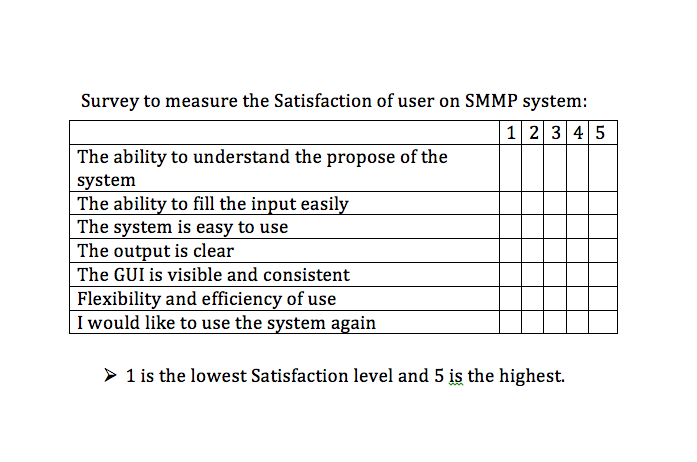
\includegraphics [width=\textwidth]{survey}
 \caption{\label{ Figure 1:} user satisfaction survey.}
 \end{center}
 \end{figure}


\end{document}
